% 勾股逆：3-4-5 直角 (古绳法)
\documentclass[tikz,border=4pt]{standalone}
\usepackage{ctex}
\usepackage{amsmath}
\begin{document}
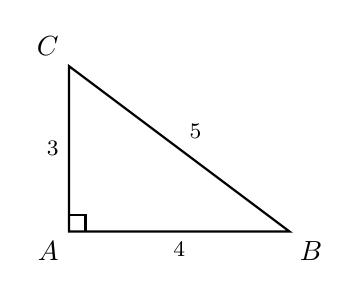
\begin{tikzpicture}[scale=0.7, thick]
  \coordinate (A) at (0,0);
  \coordinate (B) at (4,0);
  \coordinate (C) at (0,3);
  \draw (A) -- (B) -- (C) -- cycle;
  \draw (0.3,0) -- (0.3,0.3) -- (0,0.3);
  \node[below] at (2, 0) {\footnotesize $4$};
  \node[left]  at (0, 1.5) {\footnotesize $3$};
  \node[above right] at (2, 1.5) {\footnotesize $5$};
  \node[below left]  at (A) {$A$};
  \node[below right] at (B) {$B$};
  \node[above left]  at (C) {$C$};
\end{tikzpicture}
\end{document}
